% Relatório da versão 1 do software ipump para o curso
% Sistemas de Controle - DCA0206 - UFRN
% Autores:
%   AUGUSTO MATHEUS PINHEIRO DAMASCENO
%   MARCEL DA CÂMARA RIBEIRO DANTAS
%   PABLO HOLANDA CARDOSO
%   PEDRO DE CASTRO GURGEL LIMA
%   RODRIGO DANTAS DA SILVA
% Modificado por: Ícaro Bezerra Queiroz de Araújo
%

%%%%%%%%%%%% STRUCTURE %%%%%%%%%%%%%%%
\documentclass[a4paper,12pt]{article}
\usepackage[T1]{fontenc}
\usepackage[utf8]{inputenc}
\usepackage[brazil]{babel}
\usepackage{lmodern}
\usepackage{setspace}
\usepackage[top=2cm, bottom=2cm, left=2cm, right=2cm]{geometry}
%%%%%%%%%%%%%%%%%%%%%%%%%%%%%%%%%%%%%%

%%%%%%%%%%%%%%%% PAGES STYLE %%%%%%%%%
\usepackage{fancyhdr}
\fancypagestyle{main}{
\renewcommand{\headrulewidth}{0pt}
\fancyhead[RO]{\thepage}
\fancyfoot[CO]{}
}
%%%%%%%%%%%%%%%%%%%%%%%%%%%%%%%%%%%%%%

\usepackage{graphicx}
\usepackage{float}
\usepackage{epstopdf}
\usepackage{subfig}
\usepackage{mathptmx}
\usepackage{changepage}


\usepackage{listings}
\usepackage{xcolor}
\lstset{language=C++,
                basicstyle=\ttfamily,
                keywordstyle=\color{blue}\ttfamily,
                stringstyle=\color{red}\ttfamily,
                commentstyle=\color{green}\ttfamily,
                morecomment=[l][\color{magenta}]{\#}
}

%\usepackage[alf]{abntex2cite}

%%%%%%%%%%% PDF METADATA %%%%%%%%%%%%%
\usepackage[ pdftitle={MODELO RELATÓRIO},
pdfsubject={INTRODUÇÃO AO LABORATÓRIO DE CONTROLE - Grupo 3},
pdfkeywords={Controle,Automação,UFRN,DCA,ipump},
hidelinks]{hyperref}
%%%%%%%%%%%%%%%%%%%%%%%%%%%%%%%%%%%%%%

\begin{document}

\onehalfspacing

\thispagestyle{empty}

\setcounter{page}{1}

%%%%%%%%%%%% LOGOS %%%%%%%%%%%%%%%%%%%

\begin{figure}[!ht]

\centering

\subfloat{

\includegraphics[width=2.7cm]{UFRN.eps}
\label{UFRN Logo}
}
\hspace{11.09cm}
\subfloat{

\includegraphics[width=2.4cm]{DCA.eps}
\label{DCA Logo}
}

%\caption{}
\label{Logos}

\end{figure}

%%%%%%%%%%%%%%% CAPA %%%%%%%%%%%%%%%%%

\vspace{-1cm}

\begin{center}
{\bf{\normalsize UNIVERSIDADE FEDERAL DO RIO GRANDE DO NORTE\\
CENTRO DE TECNOLOGIA\\
DEPARTAMENTO DE ENGENHARIA DE COMPUTAÇÃO E AUTOMAÇÃO\\
CURSO DE ENGENHARIA DE COMPUTAÇÃO
}}


\vspace{3.6cm}

{\bf{\large RELATÓRIO DA 5ª EXPERIÊNCIA\\
CONTROLE NO ESPAÇO DE ESTADOS: OBSERVADORES DE ESTADO\\
}}
\vspace{1.5cm}
{\large TURMA: 01 A\\
	GRUPO Nº 02}


\vspace{3.6cm}


\begin{flushright}
\begin{normalsize}
ANDRESSA STÉFANY SILVA DE OLIVEIRA: 20160154101\\
\vspace{0.8cm}
FERNANDA MONTEIRO DE ALMEIDA: 20160154228\\
\vspace{0.8cm}
MÁRCIO LUIZ BEZERRA LOPES JÚNIOR: 20160154326\\
\vspace{0.8cm}
VITOR RAMOS GOMES DA SILVA: 20160154415\\
\end{normalsize}
\end{flushright}


\vspace{2.5cm}

{\large Natal-RN\\
2017}

\end{center}

\newpage

%%%%%%%%%%%%%%%  CONTRA-CAPA %%%%%%%%%

\thispagestyle{empty}

\begin{center}
\begin{normalsize}
ANDRESSA STÉFANY SILVA DE OLIVEIRA: 2016015410\\
\vspace{0.8cm}
FERNANDA MONTEIRO DE ALMEIDA 20160154228\\
\vspace{0.8cm}
MÁRCIO LUIZ BEZERRA LOPES JÚNIOR: 20160154326\\
\vspace{0.8cm}
VITOR RAMOS GOMES DA SILVA: 20160154415\\

\end{normalsize}
\end{center}
\vspace{3cm}

{\bf{\large {\centering CONTROLE NO ESPAÇO DE ESTADOS: OBSERVADORES DE ESTADO\\}}}

\vspace{4cm}

\begin{adjustwidth}{7.5cm}{0cm}

{\normalsize
Quinto relatório apresentado à disciplina de
Laboratório de Sistemas de Controle, correspondente à
avaliação da 3º unidade do semestre 2017.1 do 8º período
do curso de Engenharia de Computação da
Universidade Federal do Rio Grande do Norte, sob
orientação do {\bf Prof. Fábio Meneghetti Ugulino de
Araújo} e {\bf Prof. Lucas Costa Pereira Cavalcante.}

}

\end{adjustwidth}

\vspace{2cm}

\begin{center}

Professores:  Fábio Meneghetti Ugulino de Araújo e\\
Lucas Costa Pereira Cavalcante.

\vspace{2.5cm}

{\large Natal-RN\\
2017}

\end{center}

\newpage

%%%%%%%%%%%%%%%  RESUMO %%%%%%%%%%%%%%

\thispagestyle{empty}

\begin{center}
{\large \textbf{RESUMO}}
\end{center}

\vspace{3cm}

\begin{flushleft}

\hspace{4ex}O presente trabalho é a quinta etapa da construção de um aplicativo desktop para controle de sistema de tanques. O software utiliza a comunicação cliente/servidor no qual o sistema de tanques é o servidor. A planta antes utilizada da Quanser foi substituída por uma simulação feita em Java3D, o que eliminou o nível de ruído dos resultados. Nesta etapa do trabalho, o objetivo foi projetar e implementar um observador de estados para um controlador proporcional de segunda ordem. A teoria acerca do observador de estados é introduzida, após é apresentado os resultados dos testes de controle da planta. Por fim, chega-se a conclusão que o valor observado no tanque 2 é muito mais próximo da realidade do que o observado no tanque 1, além deste último apresentar instabilidade para polos imaginários. \\

\end{flushleft}

\vspace{1.5cm}

\textbf{Palavras-chave:} sistema de tanques; sistema de controle; software; planta Quanser, controlador PID; observação de estados, realimentação de estados.

\newpage

%%%%%%%%% LISTA DE FIGURAS %%%%%%%%%%%

\thispagestyle{empty}

\begin{center}
\listoffigures
\end{center}

\newpage

%%%%%%%%%%%%%%% SUMÁRIO %%%%%%%%%%%%%%

\thispagestyle{empty}

\begin{center}
\tableofcontents
\end{center}

\newpage

%%%%%%%%%%%%%%% INTRODUÇÃO %%%%%%%%%%%

\thispagestyle{main}

\section{INTRODUÇÃO}

%\begin{flushleft}
\hspace{4ex}A prática de laboratório 05 tem como objetivo introduzir o conceito de espaço de estados, nesse relatório será apresentado a implementação de um observador de estado para controlar o nível do tanque de baixo da planta \textit{Quanser}, sendo a figura \ref{r2d2e} a representação do simulador da planta:

\begin{figure}[H]
\centering
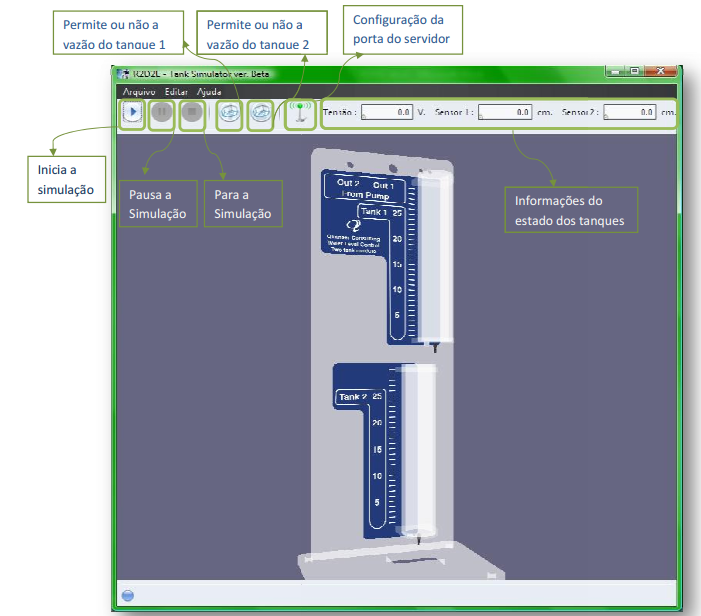
\includegraphics[width=11cm]{ImagensLab4/simulator.png}
\caption{R2D2E - Tank Simulator}
\label{r2d2e}
\end{figure}

\hspace{4ex}Essa planta é controlada através de um software desenvolvido, o qual disponibiliza opção de controle em malha aberta e malha fechada. Em malha aberta, o usuário informa a tensão que quer enviar para bomba que encherá o tanque, enquanto que em malha fechada, o valor informado será o nível do tanque. Além disso, em malha fechada, também deverá ser informado a ordem do sistema, ou seja, se o objetivo é controlar apenas o tanque de cima($L_1$) ou se o desejado é o controle do tanque de baixo($L_2$), onde nesse último caso é usado o controle em cascata. Com isso, há as opções de controle utilizando os controladores Proporcional (P), Proporcional Integrativo (PI), Proporcional Derivativo (PD), Proporcional Integrativo Derivativo (PID) e Proporcional Integrativo Derivativo em controle de ação baseado no sinal do processo (PI-D).

\hspace{4ex}E nesse laboratório, foi adicionado mais uma opção de controle, o usuário poderá escolher realizar a observação de estados, o qual será utilizado o sistema de segunda ordem em malha fechada com apenas a ação proporcional. 

\hspace{4ex}Com relação a essa última opção, na implementação do controle, foi encontrado uma representação em espaço de estados onde o nível do tanque de cima e o nível do tanque de baixo são os estados do modelo. Depois disso, a equação de estado foi discretizada utilizando o período de amostram 0,1 s.

\hspace{4ex}Na interface do software desenvolvido, o usuário deverá informar quais serão os valores dos pólos ou informar a matriz de ganhos do observador.

\begin{figure}[H]
\centering
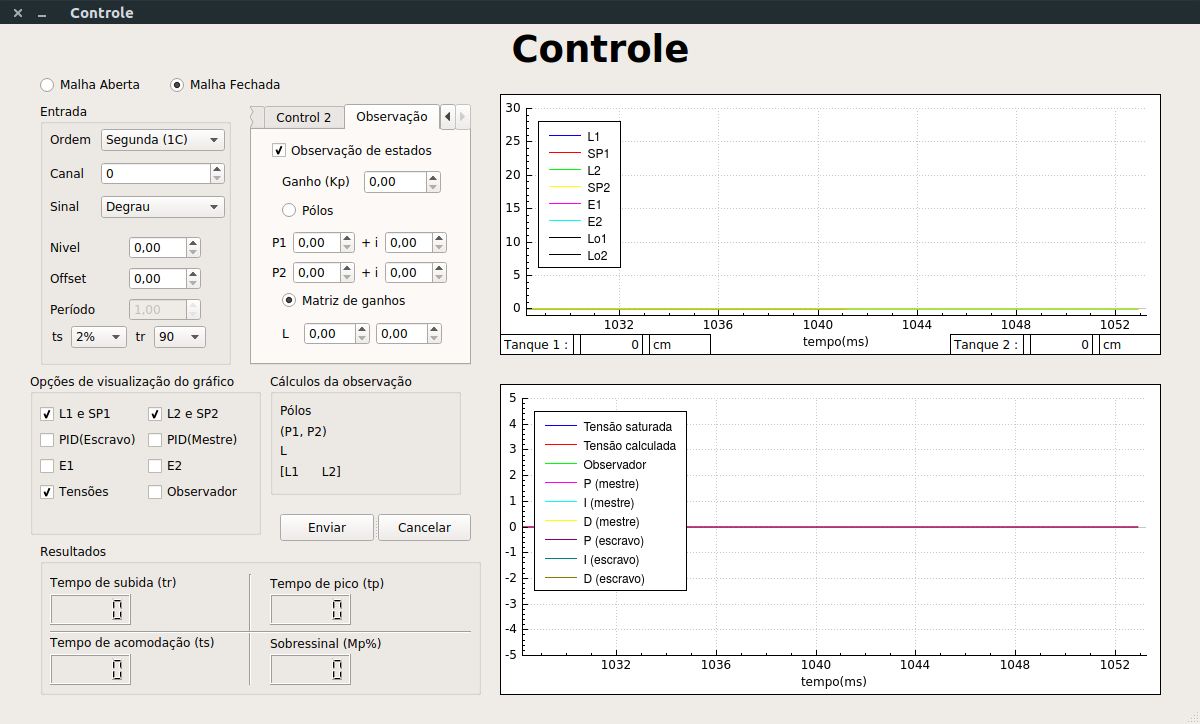
\includegraphics[width=13cm]{fotosLab5/interfaceObs.png}
\caption{Interface do software de controle}
\label{interface}
\end{figure}

\hspace{4ex}Também é possível que o usuário opte por visualizar as curvas da estimativa para cada estado e para a saída calculada a partir dos estados estimados e, assim, consiga comparar os resultados.

\hspace{4ex}Mais à frente, será abordado no relatório em que os cálculos foram baseados para a obtenção do observador de estados, a metodologia utilizada no trabalho, como também será apresentado o comportamento do observador para diferentes conjuntos de pólos e, por conseguinte, a conclusão a cerca desse controle.

%\end{flushleft}

\newpage

%%%%%%%%%% REFERENCIAL TEÓRICO %%%%%%%

\thispagestyle{main}

\section{REFERENCIAL TEÓRICO}

\subsection{DISCRETIZAÇÃO}
\hspace{4ex}Para que um computador ou microcontrolador possa controlar um sistema, estes devem ser capaz de entender as informações obtidas pelo sistema no “mundo real” de forma a trabalhar estas informações digitalmente. Mas enquanto as variáveis podem ser sinais analógicos, a máquina entende somente sinais digitais. Há, portanto, a necessidade de uma transformação nas informações recebidas pelo sistema, para que estas sejam lidas pelo controlador digital – a este processo de transformação é dado o nome de {\bf discretização}.

Em controle de estados, o comportamento do sistema será determinado por matrizes (A, B, C, D) que deverão ser modificadas uma vez que os sinais contínuos sejam discretizados, de tal forma que o comportamento do sistema discreto seja o mais próximo possível do sistema contínuo. Para encontrar as novas matrizes do sistema (G e H), aplica-se a relação entre as variáveis contínua e discreta na equação de sistemas discretos.

\begin{figure}[H]
     \centering
     \subfloat[]{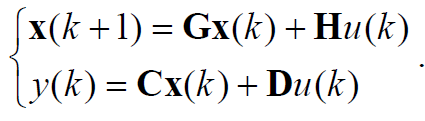
\includegraphics[width=5cm]{fotosLab5/sistema_discreto.png}\label{sistdiscreto}}
\hspace{1cm}
     \subfloat[]{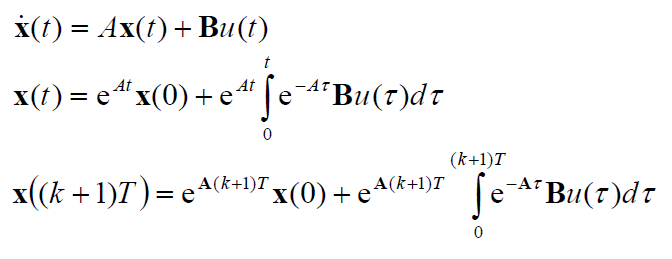
\includegraphics[width=7cm]{fotosLab5/relacao.png}\label{relacao}}
\hspace{1cm}
     \subfloat[]{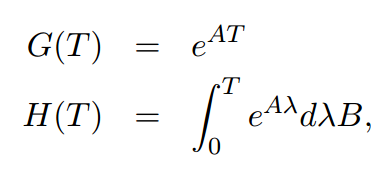
\includegraphics[width=5cm]{fotosLab5/G_H.png}\label{g_h}}
\hspace{1cm}
     \caption{G e H, matrizes do observador de tempo discreto}
     \label{fig:G_H}
\end{figure}

\subsection{OBSERVADOR DE ESTADOS}

\hspace{4ex}O observador de estados é um algoritmo que surgiu da necessidade de se medir os estados de um sistema de controle. Em função dos altos custos e às vezes da impossibilidade de se conseguir medir estes estados, o observador de estados funciona como alternativa à medição, estimando o valor das variáveis de estado através dos valores de entrada e saída.

\vspace{0.7cm}
\hspace{6ex}{\bf 1. Caso contínuo}

Supondo um sistema contínuo observável formado pelas equações:
\newpage
\begin{figure}[H]
\centering
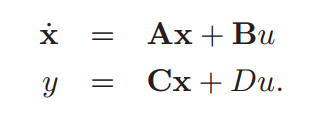
\includegraphics[width=5cm]{fotosLab5/sistema_continuo.png}
\caption{Sistema de controle contínuo}
\label{continuo}
\end{figure}

Sendo A, B, C e D conhecidos, e sendo y(t) e u(y) medidos pelo sistema, o observador de estados será definido por:

\begin{figure}[H]
\centering
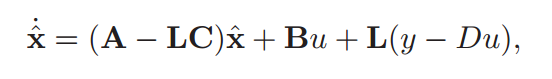
\includegraphics[width=8cm]{fotosLab5/observador_continuo.png}
\caption{Observador de estados contínuo}
\label{continuo}
\end{figure}

\vspace{0.7cm}
\hspace{6ex}{\bf 2. Caso discreto}

Supondo um sistema discreto observável, de ordem n, formado por:

\begin{figure}[h]
\centering
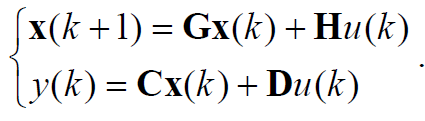
\includegraphics[width=6cm]{fotosLab5/sistema_discreto.png}
\caption{Sistema de controle discreto}
\label{sist_discreto}
\end{figure}

Sendo G, H, C e D conhecidos e sendo x(k) e u(k) obtidos pelo sistema, o observador de estados discreto será definido por:

\begin{figure}[h]
\centering
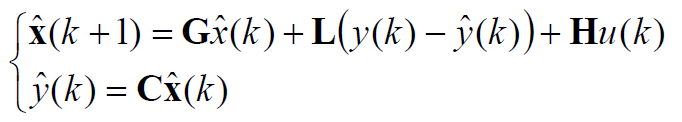
\includegraphics[width=10cm]{fotosLab5/observador_discreto.png}
\caption{Observador de estados discreto}
\label{ob_discreto}
\end{figure}

\subsubsection{ERRO DE ESTIMAÇÃO}
Erro de estimação é como é conhecida a diferença entre x e $\hat{x}$. Sabendo os valores das derivadas de x e $\hat{x}$ é possível calcular $\dot{\mathbf{e}}$:


\begin{figure}[!h]
\centering
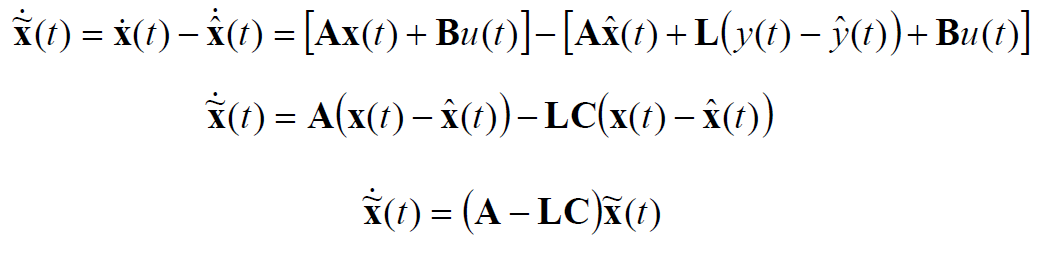
\includegraphics[width=10cm]{fotosLab5/erro_continuo.png}
\caption{Erro de estimação (tempo contínuo)}
\label{erro_continuo}
\end{figure}

Para o caso discreto, obtém-se pelo mesmo método a derivada do erro:

\begin{figure}[!h]
\centering
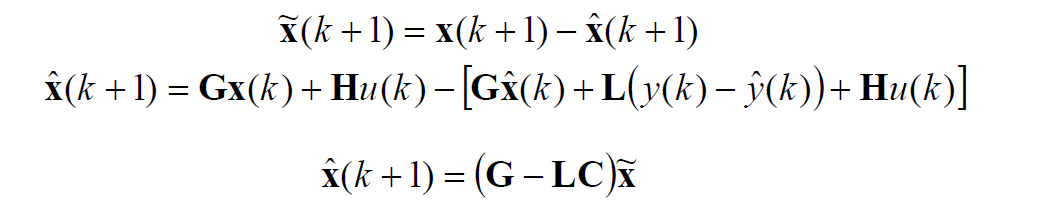
\includegraphics[width=10cm]{fotosLab5/erro_discreto.png}
\caption{Erro de estimação (tempo discreto)}
\label{erro_discreto}
\end{figure}

\subsubsection{FÓRMULA DE ACKERMANN}

\hspace{4ex}A fórmula de Ackermann permite determinar através de variáveis conhecidas o vetor de ganhos do sistema.

O vetor de ganhos terá o formato:

\hspace{4ex}{\bf L=[L1,L2,…,Ln]}

Os elementos dos vetores serão encontrados pela fórmula de Ackermann. Para o caso discreto, teremos:

\begin{figure}[!h]
\centering
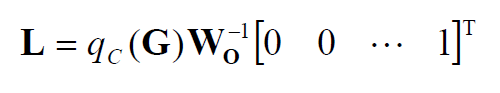
\includegraphics[width=5cm]{fotosLab5/ackermann.png}
\caption{Fórmula de Ackermann}
\label{ackermann}
\end{figure}


\newpage
%%%%%%%%%% METODOLOGIA %%%%%%%%%%%%%%%



\section{METODOLOGIA}

\hspace{4ex}Para se fazer a observação de estados da planta, foi necessário obter as matrizes G e H. A partir do modelo oferecido na descrição do experimento, pode-se calcular com as estratégias citadas anteriormente, na seção Referencial Teórico. Além de obter essas matrizes, foi verificado se o sistema é observável, e foi obtido um resultado positivo. Juntamente com esse cálculo, de forma análoga, observou que o sistema não é controlável.

\hspace{4ex}Uma vez com as informações importantes do sistema, a implementação da observação de estados se transforma em algoritmos de cálculo de pólos e cálculo da matriz de ganhos L. Feitas nos seguintes métodos.

\begin{lstlisting}

vector<complex<double>> Observador::Calcula_Polos(Matriz ll)
{
    complex<double> a00(G[0][0],0), a01(G[0][1],0), 
    		a10(G[1][0],0), a11(G[1][1],0);
    complex<double> l1(ll[0][0],0), l2(ll[1][0],0);
    vector<complex<double>> polos;
    complex<double> p1= -(-a00-a11+l2+
    	sqrt(pow(l2,2)+(2.0*a00-2*a11)*l2-4.0*a10*l1+
    	pow(a11,2.0)-2.0*a00*a11+
    	4.0*a01*a10+pow(a00,2)))/2.0;
    complex<double> p2=  (a00+a11-l2+
    	sqrt(pow(l2,2)+(2.0*a00-2.0*a11)*l2-4.0*a10*l1+
    	pow(a11,2)-2.0*a00*a11+4.0*a01*a10+pow(a00,2)))/2.0;
    polos.push_back(p1);
    polos.push_back(p2);
    return polos;
}
Matriz Observador::Calcula_L(complex<double> p1, complex<double> p2)
{
    Matriz I= Matriz::Identidade(2), aux(2,1);
    aux[0][0]= 0;
    aux[1][0]= 1;
    double c[2]= {(-p1-p2).real(), (p1*p2).real()};
    Matriz Ackerman= (G^2)+(c[0]*G)+(c[1]*I);
    L= (Ackerman*W_inv)*aux;
    return L;
}


\end{lstlisting}
\hspace{4ex}Os métodos acima, são algoritmos que representam os cálculos citados no referencial teórico. Já no método para encontrar os pólos, foi feito uma manipulação algébrica a partir das equações para encontrar a matriz L.

\hspace{4ex}Tais cálculos são feitos devido o programa ter como entrada os pólos e a matriz de ganhos, como mostrado na figura a seguir. Quando o usuário escolhe inserir o pólos, é feita a chamada do método Calcula\_L, para então observar o sistema.

\begin{figure}[H]
     \centering
     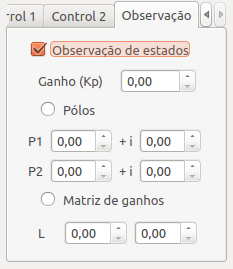
\includegraphics[width=4cm]{fotosLab5/observador-interface}}
     \caption{Interface referente as entradas da observação}
     \label{fig:obs-inter}
\end{figure}

\hspace{4ex}Caso contrário, ou seja, caso a entrada seja a matriz L, é encontrado os pólos e apresentado ao usuário na interface os respectivos pólos.

\hspace{4ex}Por fim, utilizando o simulador R2D2E, foram feitos testes de controle fixado no tipo proporcional para o sistema de segunda ordem com apenas um controlador, alternando entre as opções dadas ao usuário, ora tendo como entrada os pólos, ora a matriz L. Sendo que o foco foi o teste com vários pólos, pois desejava-se encontrar os pólos mais adequados para o sistema. 




\newpage

%%%%%%%%%% RESULTADOS %%%%%%%%%%%%%%%

\thispagestyle{main}

\section{RESULTADOS}
\hspace{4ex}Nas figuras a seguir será apresentado os gráficos da interface do software, a qual mostrará o comportamento do observador de estados para vários pólos, onde a curva em azul indica o nível do tanque 1($L_1$), a curva em verde é o nível do tanque 2($L_2$), a curva em preto é o nível observado do tanque 1 e a curva em cinza é o nível observado do tanque 2.

\hspace{4ex}Inicialmente, como mostrado nas figuras \ref{img1} e \ref{img2}, foi inserido dois pólos em 0, logo, é possível observar que a curva do nível do tanque 2 ficou alinhada com a curva informada pelo sensor, isso indica que seus valores estão muito próximos, enquanto que no tanque 1, pode-se perceber que o valor estimado do nível se aproxima do valor real, mas o ultrapassa, pois  o observador está muito rápido devido aos pólos na origem.
\begin{figure}[!h]
\centering
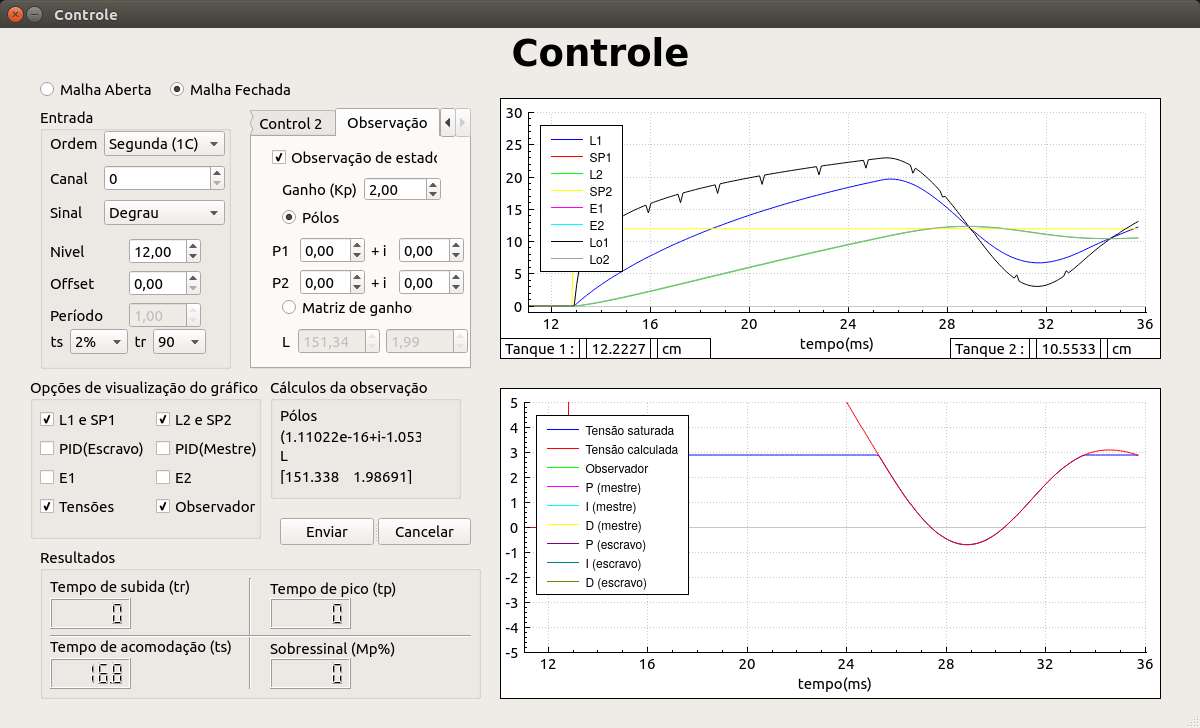
\includegraphics[width=13cm]{FotosObservador/PolosEm01}
\caption{Observador com dois polos em 0}
\label{img1}
\end{figure}
\begin{figure}[!h]
\centering
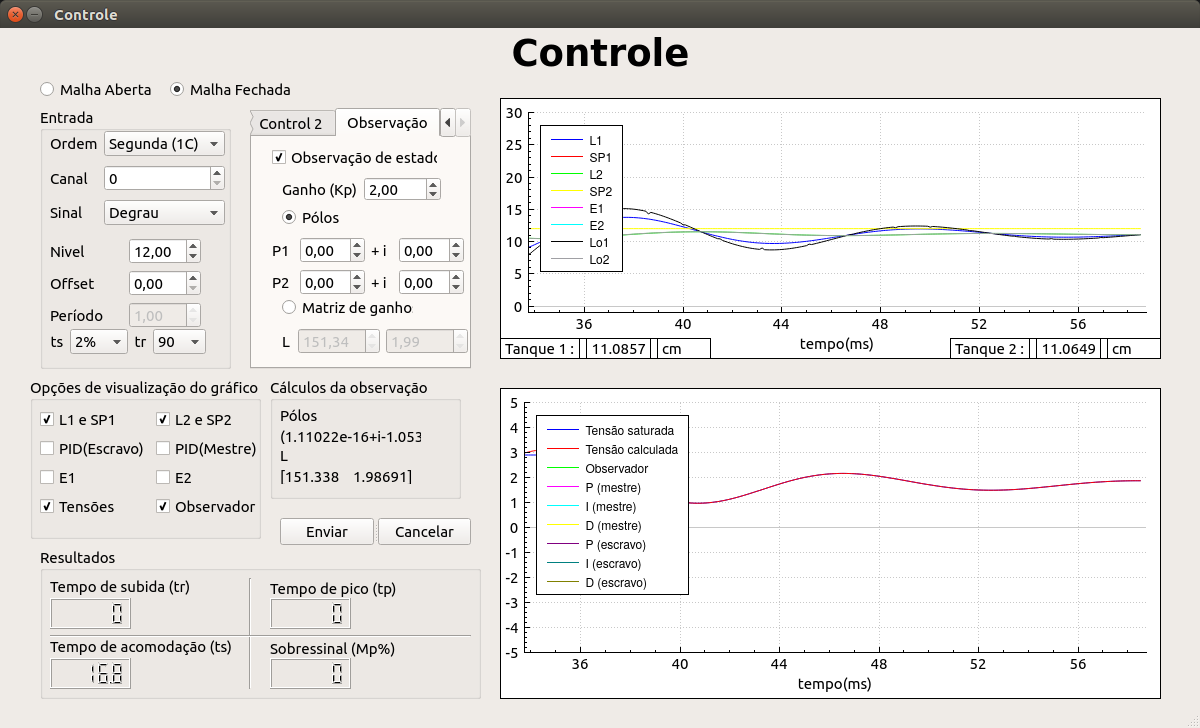
\includegraphics[width=13cm]{FotosObservador/PolosEm02}
\caption{Observador com dois pólos em 0}
\label{img2}
\end{figure}

\hspace{4ex}Agora com pólos imaginários em 0.7+0.7i e 0.7-0.7i, o valor observado do tanque 1 foi bastante oscilatório, como esperado, e o valor do tanque 2 contínuo, ou seja, a curvado observável acompanhando a curva real do nível, verifique as figuras \ref{img3} e \ref{img4}.
\begin{figure}[!h]
\centering
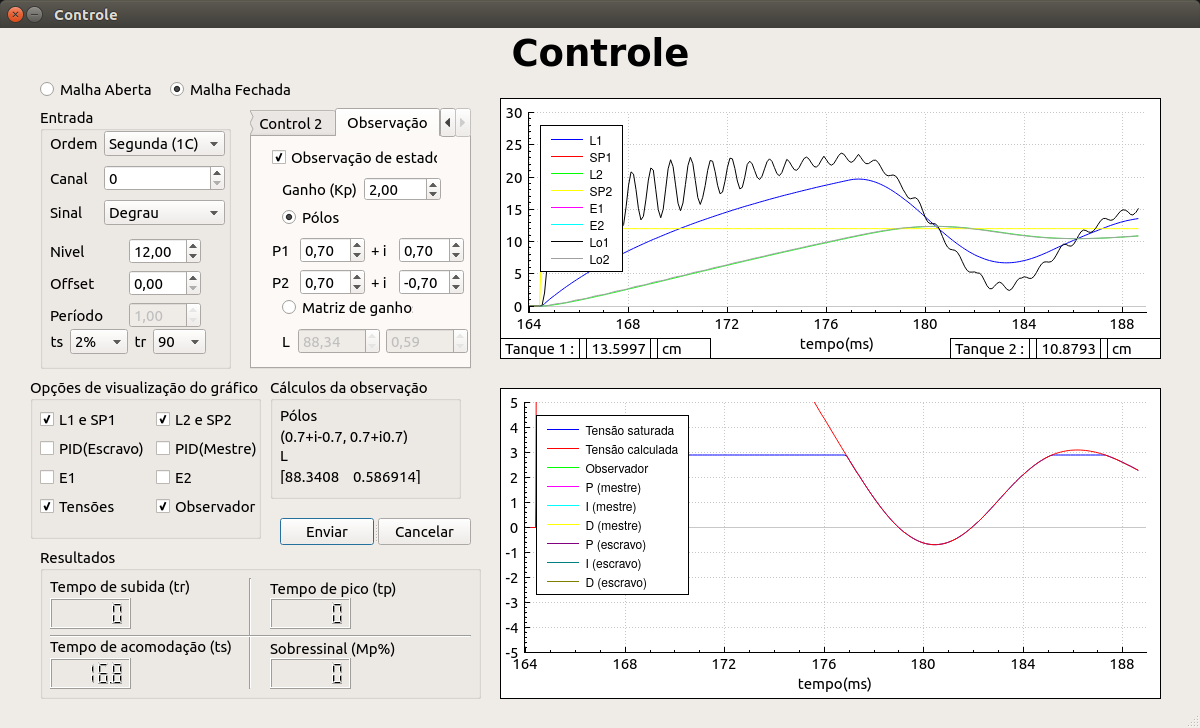
\includegraphics[width=13cm]{FotosObservador/PoloImaginario2}
\caption{Observador com pólos imaginários}
\label{img3}
\end{figure}
\begin{figure}[!h]
\centering
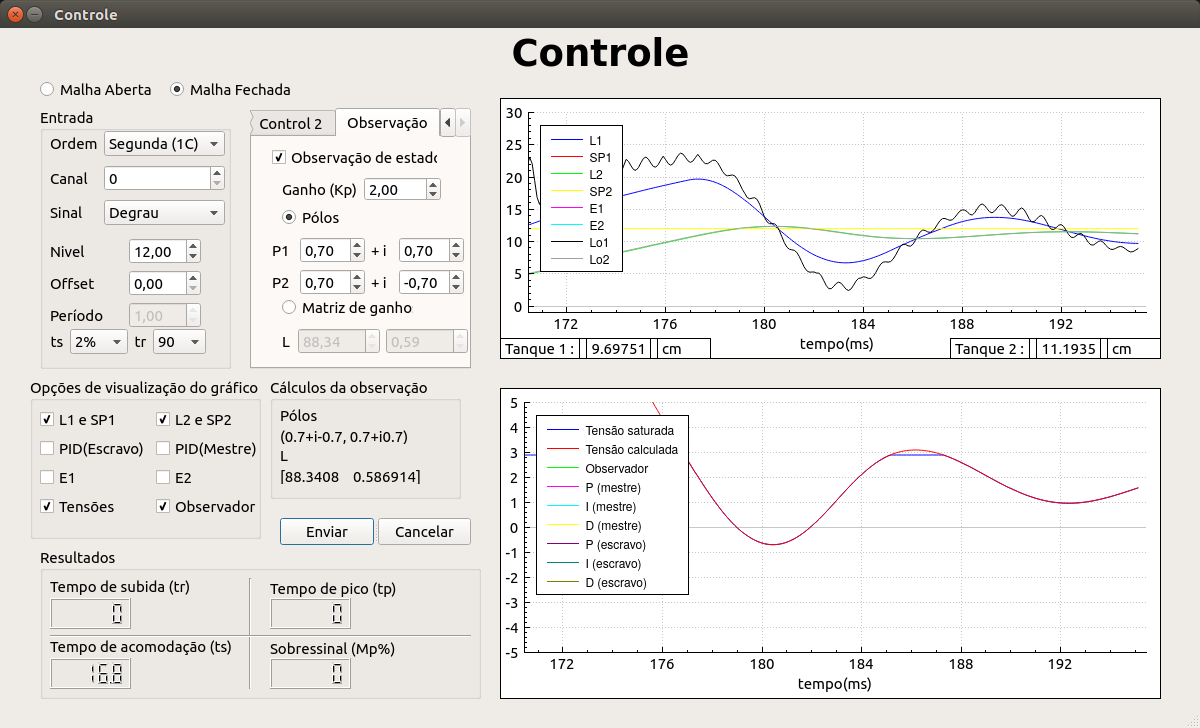
\includegraphics[width=13cm]{FotosObservador/PoloImaginario1}
\caption{Observador com pólos imaginários}
\label{img4}
\end{figure}

\newpage
\hspace{4ex}Depois disso, com dois pólos reais distantes do centro da circuferência, em 0.99 e 0.99, nota-se que até mesmo o nível do tanque 2 demora para acompanhar o valor real da curva, observe as figuras \ref{img5} e \ref{img6}.
\begin{figure}[!h]
\centering
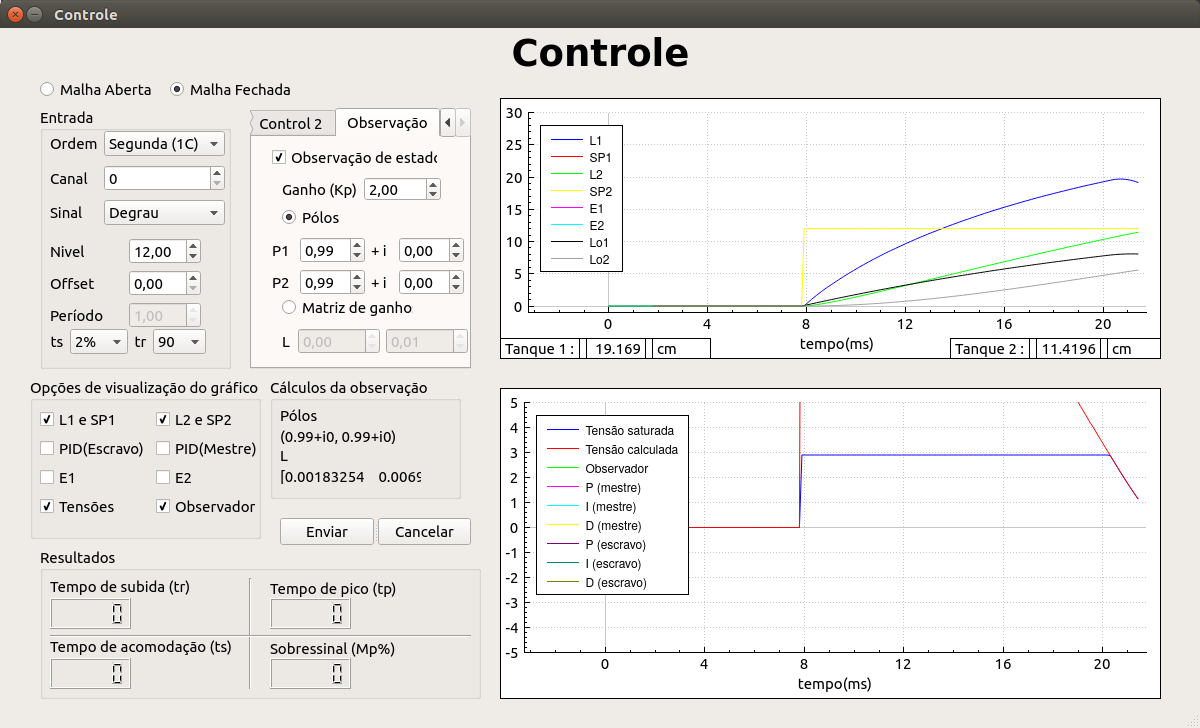
\includegraphics[width=13cm]{FotosObservador/PolosMuitoLentos1}
\caption{Observador com pólos distantes da origem}
\label{img5}
\end{figure}
\begin{figure}[!h]
\centering
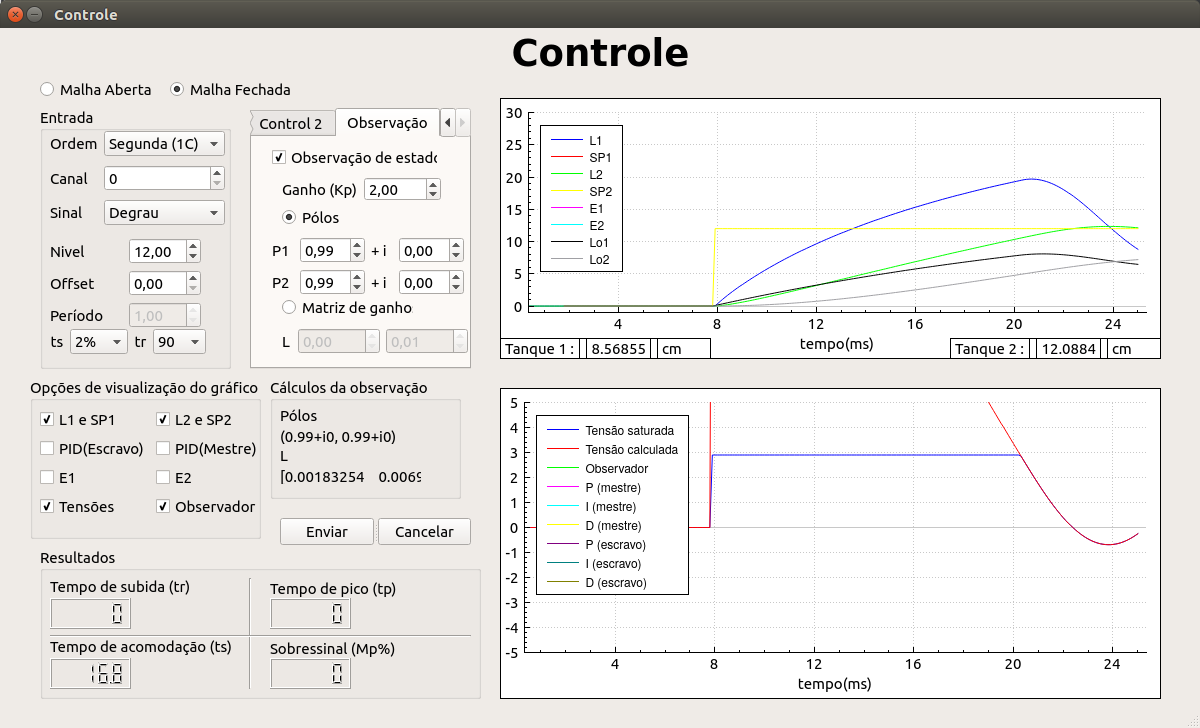
\includegraphics[width=13cm]{FotosObservador/PolosMuitoLentos2}
\caption{Observador com pólos distantes da origem}
\label{img6}
\end{figure}

\newpage
\hspace{4ex}Por fim, foi utilizado pólos reais, um na origem e outro distante da origem, em 0.99, nessa configuração ambos os valores estimados foram bons. Na figura \ref{img7}, o tempo de subida foi pequeno e, na figura \ref{img8}, o tempo de subida foi grande.
\begin{figure}[!h]
\centering
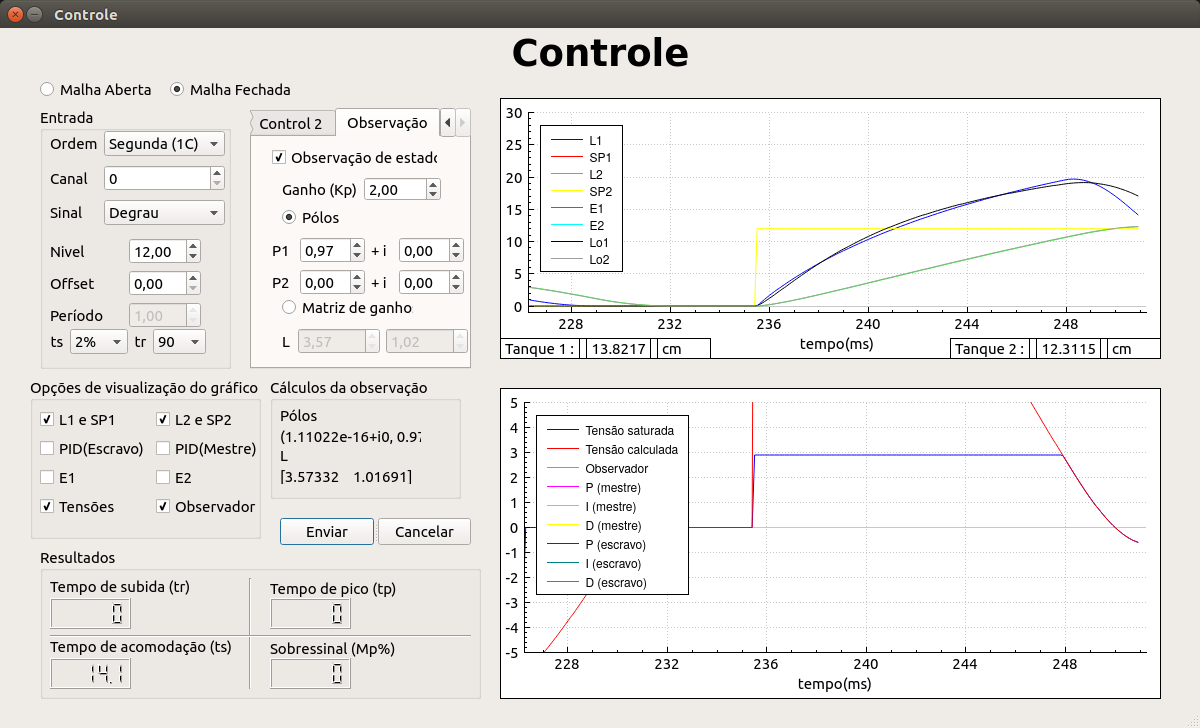
\includegraphics[width=13cm]{FotosObservador/PoloRapidoELento2}
\caption{Observador com um pólo na origem e outro distante}
\label{img7}
\end{figure}
\begin{figure}[!h]
\centering
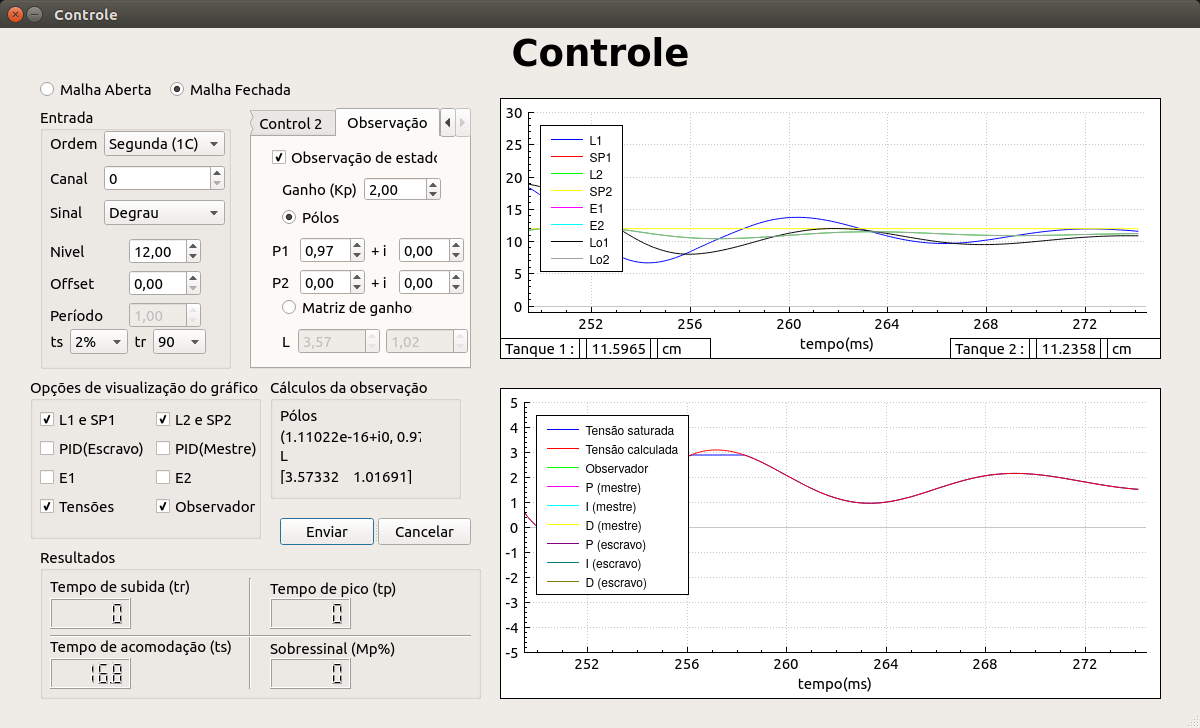
\includegraphics[width=13cm]{FotosObservador/PoloRapidoELento1}
\caption{Observador com um pólo na origem e outro distante}
\label{img8}
\end{figure}

\newpage

%%%%%%%%%% CONCLUSÃO %%%%%%%%%%%%%%%

\thispagestyle{main}

\section{CONCLUSÃO}

\hspace{4ex}A partir dos testes realizados com os pólos em zero, pólos imaginários e pólos reais, pode-se concluir que o observador de estados mostrou que o valor observado do tanque 2 será semelhante e, muitas vezes, igual ao valor real do nível, enquanto que o valor observável do tanque 1 foi uma aproximação. Além disso, no caso dos pólos imaginários em particular, o nível observável do tanque 1 se mostrou muito oscilatório com relação ao seu valor real.

\newpage
%%%%%%%% REFERÊNCIAS %%%%%%%%%%%%%%%%%

\thispagestyle{empty}
\section{BIBLIOGRAFIA}

Fundamentals of cascade control | Control Engineering. Disponível em: <http://www.controleng.com/single-article/fundamentals-of-cascade-control/bcedad6518aec409f583ba6bc9b72854.html>. Acesso em: 10 maio. 2017.




%Referências bibliogáficas (geradas automaticamente)

%\addcontentsline{toc}{chapter}{Referências bibliográficas}
%\bibliography{bib/bibliografia}

%\appendix

%Apêndice A
%\include{apendice}

\end{document}
